% !TeX encoding = UTF-8
% !TeX spellcheck = en_AU
% !TeX root = TNLectureNotes.tex

\RequirePackage[l2tabu, orthodox]{nag}

\usepackage[margin=20mm]{geometry}
\usepackage[numbib,nottoc]{tocbibind}
\usepackage{etex,amsmath,amsfonts,array,mathtools,tikz,xcolor,color,graphicx,amssymb,amsthm,bm,bbm,pgfplots,mdframed,complexity,blkarray,thmtools,forloop,ifthen,titlepic,soul}
\usepackage{placeins}
\usepackage{cite,xr-hyper}

\definecolor{tensorblue}{rgb}{0.8,0.8,1}
\definecolor{tensorred}{rgb}{1,0.5,0.5}
\definecolor{tensorpurp}{rgb}{1,0.5,1}

\tikzset{ten/.style={fill=tensorblue}}
\tikzset{tenred/.style={fill=tensorred}}
\tikzset{tengreen/.style={fill=green!50!black!50}}
\tikzset{tenpurp/.style={fill=tensorpurp}}
\tikzset{tengrey/.style={fill=black!20}}
\tikzset{tenorange/.style={fill=orange!30}}
\tikzset{u/.style={fill=blue!20,draw=black}}
\tikzset{w/.style={fill=green!50!black!80,draw=black}}

\DeclareMathOperator{\Cont}{Cont} 

\makeatletter
\newcommand{\rmnum}[1]{\romannumeral #1}
\newcommand{\Rmnum}[1]{\expandafter\@slowromancap\romannumeral #1@}
\makeatother

\newcommand{\tikzname}[1]{
\ifthenelse{\COMPILETIKZ=1}
{\stepcounter{TikzExternaliseName}\tikzsetnextfilename{Tikz\theTikzExternaliseName}
	#1}
{\stepcounter{TikzExternaliseName}\includegraphics{./figures/\tikzsubfolder/Tikz\theTikzExternaliseName.pdf}}}

\newcommand{\diagram}[1]{ \begin{array}{cc}\tikzname{\begin{tikzpicture}[scale=.5,every node/.style={sloped,allow upside down},baseline={([yshift=+0ex]current bounding box.center)}] #1 \end{tikzpicture}} \end{array} }

\newcommand{\diagramsized}[2]{ \begin{array}{cc} \tikzname{\begin{tikzpicture}[scale=#1,every node/.style={sloped,allow upside down},baseline={([yshift=+0ex]current bounding box.center)}] #2 \end{tikzpicture}} \end{array} }
\definecolor{awesome}{rgb}{0.33, 0.42, 0.18}
\usepackage{hyperref}
\hypersetup{citecolor=violet}
\hypersetup{linkcolor=red}
\hypersetup{urlcolor=blue}
\hypersetup{filecolor=awesome}
\hypersetup{colorlinks=true}
\hypersetup{pdfborder={0 0 0}}
\usepackage[capitalise]{cleveref}


\pgfplotsset{compat=newest}
\pgfplotsset{plot coordinates/math parser=false}
\usetikzlibrary{arrows,decorations.pathmorphing,backgrounds,positioning,fit,calc,patterns,shapes,external}
\tikzexternalize[prefix=figures/\tikzsubfolder/]


\numberwithin{equation}{section}

\newtheorem{lemma}{Lemma}
\newtheorem{theorem}{Theorem}
\newtheorem{claim}{Claim}[section]

\renewenvironment{proof}[1][Proof]{\noindent\textbf{#1.} }{\ $\Box$}

\def\N{\mathbb{N}}
\def\Z{\mathbb{Z}}
\def\R{\mathbb{R}}
\def\C{\mathbb{C}}
\def\Q{\mathbb{Q}}
\def\F{\mathbb{F}}
\def\E{\mathbb{E}}

\def\e{\mathrm{e}}

\newcommand{\Eref}[1]{Eq.~(\ref{#1})}
\newcommand{\Sref}[1]{Sec.~\ref{#1}}
\newcommand{\Fref}[1]{Fig.~\ref{#1}}
\newcommand{\Aref}[1]{Appendix~\ref{#1}}

%\let\oldonlinecite\onlinecite

\def\eps{\epsilon}
\def\veps{\varepsilon}
\def\cO{\mathcal{O}}
\DeclareMathOperator{\Tr}{Tr}
\DeclareMathOperator{\tr}{tr}

\newcommand{\ket}[1]{|{#1}\rangle}
\newcommand{\expect}[1]{\langle{#1}\rangle}
\newcommand{\bra}[1]{\langle{#1}|}
\newcommand{\ketbra}[2]{|{#1}\rangle\!\langle{#2}|}
\newcommand{\braket}[2]{\langle{#1}|{#2}\rangle}
\newcommand{\proj}[1]{\ketbra{#1}{#1}}
\newcommand{\vket}[1]{|{#1})}
\newcommand{\braopket}[3]{\left\langle #1\middle|#2\middle|#3\right\rangle}

\newcommand*{\one}{\mathbbm{1}} % identity

\newcommand{\norm}[1]{\left\lVert#1\right\rVert}
\newcommand{\comm}[1]{\left[#1\right]}

\newcommand{\rx}[1]{\textcolor{red}{X_{#1}^{(1)}}}
\newcommand{\ry}[1]{\textcolor{red}{Y_{#1}^{(1)}}}
\newcommand{\rz}[1]{\textcolor{red}{Z_{#1}^{(1)}}}

\newcommand{\bx}[1]{\textcolor{blue}{X_{#1}^{(2)}}}
\newcommand{\by}[1]{\textcolor{blue}{Y_{#1}^{(2)}}}
\newcommand{\bz}[1]{\textcolor{blue}{Z_{#1}^{(2)}}}

\newcommand{\midarrow}{\tikz \draw[-triangle 90] (0,0) -- +(.1,0);}

\newcommand{\MPOtensor}[3]{
\def\a{#1}
\def\dx{#2}
\def\x{#3}
\draw[shift={(\x*\a+\x*\dx,0)}] (-\dx/2,0) -- (0,0);
\filldraw[a,shift={(\x*\a+\x*\dx,0)}] (0,0) -- (\a/2,\a/2) -- (\a,0) -- (\a/2,-\a/2) -- (0,0);
\draw[shift={(\x*\a+\x*\dx,0)}] (\a,0) -- (\a+\dx/2,0);
\draw[shift={(\x*\a+\x*\dx,0)}] (\a/2,\a/2) -- node {\midarrow}(\a/2,\a/2+\dx/2);
\draw[shift={(\x*\a+\x*\dx,0)}] (\a/2,-\a/2-\dx/2) -- node {\midarrow} (\a/2,-\a/2);
}

\newcommand{\drawpeps}{\tikzname{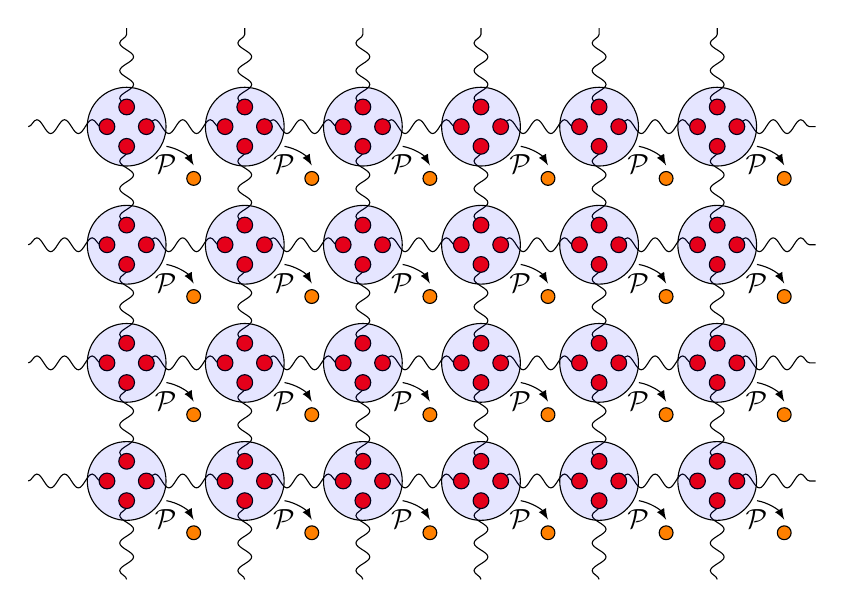
\begin{tikzpicture}[a/.style={fill=red,fill opacity = 1},scale=.5,every node/.style={sloped,allow upside down},baseline={([yshift=-.8ex]current bounding box.center)},
ent/.style={decorate,decoration={snake,segment length=10}},
b/.style={fill=blue,fill opacity = .1,text opacity=1} ]
\def\a{2}
\def\dx{1}
\def\dy{1}
\foreach \x in {0,1,...,6}{
    	\foreach \y in {0,1,...,4}{
    		\ifthenelse{\y<4}{
    			\draw[ent,shift={(\x*\a+\x*\dx-\a-\dx/2,\y*\a+\y*\dy)}] (0,0)--(\a,0);
    		};
    		\ifthenelse{\x<6}{
    			\draw[ent,shift={(\x*\a+\x*\dx,\y*\a+\y*\dy-\a-\dy/2)}] (0,0)--(0,\a);
    		};
    	}
}
\foreach \x in {0,1,...,5}{
    \foreach \y in {0,1,...,3}{
    	\filldraw[a,shift={(\x*\a+\x*\dx-\dx/2,\y*\a+\y*\dy)}] (0,0) circle (.2);
    	\filldraw[a,shift={(\x*\a+\x*\dx+\dx/2,\y*\a+\y*\dy)}] (0,0) circle (.2);
    	\filldraw[a,shift={(\x*\a+\x*\dx,\y*\a+\y*\dy+\dy/2)}] (0,0) circle (.2);
    	\filldraw[a,shift={(\x*\a+\x*\dx,\y*\a+\y*\dy-\dy/2)}] (0,0) circle (.2);
	}
}
\foreach \x in {0,1,...,5}{
	\foreach \y in {0,1,...,3}{
    	\filldraw[b,shift={(\x*\a+\x*\dx,\y*\a+\y*\dy)}] (0,0) circle (\dx) node[below right = \dx/3] {$\mathcal{P}$};
    	 \draw [-latex,shift={(\x*\a+\x*\dx+1.0\dy,\y*\a+\y*\dy-\dx/2)}] (0,0) arc [radius=\dx, start angle=80, end angle= 30]node[draw,below=2pt,circle,minimum size=5pt,fill=orange,inner sep=0pt]{};
    }
}
  \end{tikzpicture}}}

\def\Put(#1,#2)#3{\leavevmode\makebox(0,0){\put(#1,#2){#3}}}

\makeatletter
\renewcommand*\env@matrix[1][\arraystretch]{%
  \edef\arraystretch{#1}%
  \hskip -\arraycolsep
  \let\@ifnextchar\new@ifnextchar
  \array{*\c@MaxMatrixCols c}}
\makeatother

\declaretheoremstyle[
spaceabove=\topsep, spacebelow=\topsep,
notefont=\mdseries\bfseries, notebraces={}{},
headformat={\NAME\,\,\NUMBER\,:\,\if\NOTE \else \NOTE\fi},
bodyfont=\normalfont,
postheadspace={\newline},
headpunct=\newline,
numberwithin=,
preheadhook={
	%\vspace{-5cm}
	\begin{mdframed}[backgroundcolor=blue!5, %
	innertopmargin =0pt , splittopskip = \topskip, % 
	innerbottommargin =1eX, % 
	skipbelow= 6pt, skipabove=6pt,linecolor=blue!20,linewidth=2pt]},
postheadhook={\hspace*{\parindent}},
postfoothook={\end{mdframed}\vspace{.5cm}}
]{aside}
\declaretheorem[style=aside]{aside}
\crefname{aside}{Aside}{Asides}

\declaretheoremstyle[
spaceabove=\topsep, spacebelow=\topsep,
notefont=\mdseries\bfseries, notebraces={}{},
bodyfont=\normalfont,
headpunct=\newline,
numberwithin=,
preheadhook={
	%\vspace{-.5cm}
	\begin{mdframed}[backgroundcolor=blue!5, %
	innertopmargin =0pt , splittopskip = \topskip, % 
	innerbottommargin =1eX, % 
	skipbelow= 6pt, skipabove=6pt,linecolor=blue!20,linewidth=2pt]},
postheadhook={\hspace*{\parindent}},
postfoothook={\end{mdframed}\vspace{.5cm}}
]{soln}
\declaretheorem[style=soln]{soln}
\crefname{soln}{Soln}{Solns}

\externaldocument[Sol-]{./TNSolutions}
\newcommand{\solref}[1]{\ref*{Sol-#1}}

\declaretheoremstyle[
spaceabove=\topsep, spacebelow=\topsep,
notefont=\mdseries\bf, notebraces={}{},
headformat={},
bodyfont=\normalfont,
postheadspace=\newline,
headpunct=,
numberwithin=,
preheadhook={
	\vspace{1cm}
	\refstepcounter{subsection}
	\addcontentsline{toc}{subsection}{\protect\numberline{\thesubsection}Problems}
	\begin{mdframed}[backgroundcolor=red!5, %
  innertopmargin =0pt , splittopskip = \topskip, % 
  innerbottommargin =1eX, % 
  skipbelow= 6pt, skipabove=6pt,linecolor=red!20,linewidth=2pt]
  \subsection*{Problems \protect\numberline{\thesection}}
	Solutions in accompanying document.  %(\hyperref[Sol-s:sols\thesection]{Solutions \thesection})
  \vspace{-1cm}
  },
 postheadhook={\hspace*{\parindent}\begin{enumerate}},
postfoothook={\end{enumerate}\end{mdframed}}
]{problems}
\declaretheorem[style=problems]{problems}
\crefname{problem}{Problem}{Problems}

\declaretheoremstyle[
spaceabove=\topsep, spacebelow=\topsep,
notefont=\mdseries\bf, notebraces={}{},
headformat={},
bodyfont=\normalfont,
postheadspace=\newline,
headpunct=,
numberwithin=,
preheadhook={\label{s:sols\thesection}
	\vspace{1cm}
	\refstepcounter{subsection}
	\begin{mdframed}[backgroundcolor=red!5, %
  innertopmargin =0pt , splittopskip = \topskip, % 
  innerbottommargin =1eX, % 
  skipbelow= 6pt, skipabove=6pt,linecolor=red!20,linewidth=2pt]
  \subsection*{Solutions \protect\numberline{\thesection}}
  \vspace{-1cm}
  },
 postheadhook={\hspace*{\parindent}\begin{enumerate}},
postfoothook={\end{enumerate}\end{mdframed}}
]{problems_sol}
\declaretheorem[style=problems_sol]{problems_sol}
\crefname{problem}{Problem}{Problems}

\makeatletter
\renewenvironment{thebibliography}[1]
{\subsection{References}% <-- this line was changed from \chapter* to \section*
	\@mkboth{\MakeUppercase\bibname}{\MakeUppercase\bibname}%
	\list{\@biblabel{\@arabic\c@enumiv}}%
	{\settowidth\labelwidth{\@biblabel{#1}}%
		\leftmargin\labelwidth
		\advance\leftmargin\labelsep
		\@openbib@code
		\usecounter{enumiv}%
		\let\p@enumiv\@empty
		\renewcommand\theenumiv{\@arabic\c@enumiv}}%
	\sloppy
	\clubpenalty4000
	\@clubpenalty \clubpenalty
	\widowpenalty4000%
	\sfcode`\.\@m}
{\def\@noitemerr
	{\@latex@warning{Empty `thebibliography' environment}}%
	\endlist}
\makeatother

\usepackage[sectionbib]{chapterbib}

\allowdisplaybreaks

\renewcommand{\abstractname}{}

\newcounter{TikzExternaliseName}

\usepackage{currfile}
\usepackage{arydshln}


\hypersetup{
	pdfinfo={
		Title={Hand-waving and Interpretive Dance},
		Author={J.C.\ Bridgeman and C.T.\ Chubb},
	}
}

%\newcommand{\add}[1]{{\color{blue}\bf #1}}
%\newcommand{\del}[1]{{\color{red}\it{#1}}}
\newcommand{\add}[1]{#1}
\newcommand{\del}[1]{}